\section{Grundlagen von Expertensystemen}\label{sec:Grundlagen}
\subsection{Begriffsdefinition}\label{subsec:Begriffsdefinition}
Urspr�nglich waren Expertensysteme Anwendungsprogramme, die logische Schlussfolgerungen aus einer Wissensbasis ziehen konnten. Au�erdem konnten sie �berpr�fen, ob eine Aussage aus einer vorhandenen Wissensbasis abgeleitet werden kann \cite[S.75]{greer2010}. Daher handelt es sich in der fr�heren Literatur meist um Anwendungen, die ihr Wissen in Form von logischen Ausdr�cken darstellen und in der Lage waren, neue Erkenntnisse vom bestehenden Wissen abzuleiten \cite{tecuci1992}. Im Laufe der Zeit hat sich das Konzept eines Expertensystems auf andere Anwendungsbereiche verbreitet. Aus diesem Grund gibt es mehrere Definitionen, die im Allgemeinen �hnlich sind und im Spezifischen Merkmale des zugeh�rigen Anwendungsbereichs beinhalten.\\
Allgemein l�sst sich sagen, dass ein Expertensystem ein Computersystem (Hardware und Software) ist, das in einem bestimmten Bereich Wissen und Schlussfolgerungsf�higkeit eines menschlichen Experten nachbildet \cite[S.12]{beierle2014}. Aus Sicht der Wirtschaftsinformatik zielen Expertensysteme drauf ab, das Expertenwissen menschlicher Fachleute in der Wissensbasis eines Computers abzuspeichern und f�r eine Vielzahl von Probleml�sungen zu nutzen \cite[S.59]{mertens2012}. Im Weiteren gehen Beierle und Kern-Isberner auf die Eigenschaften ein, die ein Expertensystem aufweisen soll \cite[S.12]{beierle2014}. Im Rahmen dieser Arbeit sind folgende Eingenschaften besonders relevant:
\begin{itemize}
\item Anwendung des Wissens eines oder mehrerer Experten, um Probleme in einem bestimmten Anwendungsbereich zu l�sen.
\item Leicht lesbare Wissensdarstellung.
\item M�glichst anschauliche und intuitive Benutzerschnittstelle.
\item Leichte Wartbarkeit und Erweiterbarkeit des Wissens im Expertensystem.
\item Unterst�tzung beim Wissenstransfer vom Experten zum System.
\end{itemize}
Es ist auch wichtig anzumerken, dass die Begriffe \grqq{}K�nstliche Intelligenz\grqq{}, \grqq{}Wissensbasiertes System\grqq{} und \grqq{}Expertensystem\grqq{} in einer engen Beziehung zueinander stehen. Haun gibt eine systematische Abgrenzung dieser Begriffe, die sich folgenderma�en beschreiben l�sst \cite[S.30]{haun2000}:
\begin{itemize}
\item \textit{K�nstliche Intelligenz} stellt den Oberbegriff dar und bildet den theoretischen Rahmen f�r die Entwicklung von Wissensbasierten Systemen und Expertensystemen.
\item \textit{Wissensbasierte Systeme} sind eine Teilmenge der Anwendungen der k�nstlichen Intelligenz. Sie wenden die Wissensverarbeitung auf ein konkretes Aufgabengebiet an und verwalten Allgemeinwissen explizit und getrennt vom Rest des Systems.
\item \textit{Expertensysteme}, die ein Teilbereich der Wissensbasierten Systeme sind, stellen eine Spezialisierung von Wissensbasierten Systemen dar. Sie verwalten spezifisches Expertenwissen, das von einem Experten stammt und auf praxisbezogene Probleme angewandt wird.
\end{itemize}
Graphisch l�sst sich die vorliegende Abgrenzung in der Abbildung \ref{Abgrenzung} darstellen:
\begin{figure}[H] 
	\centering
	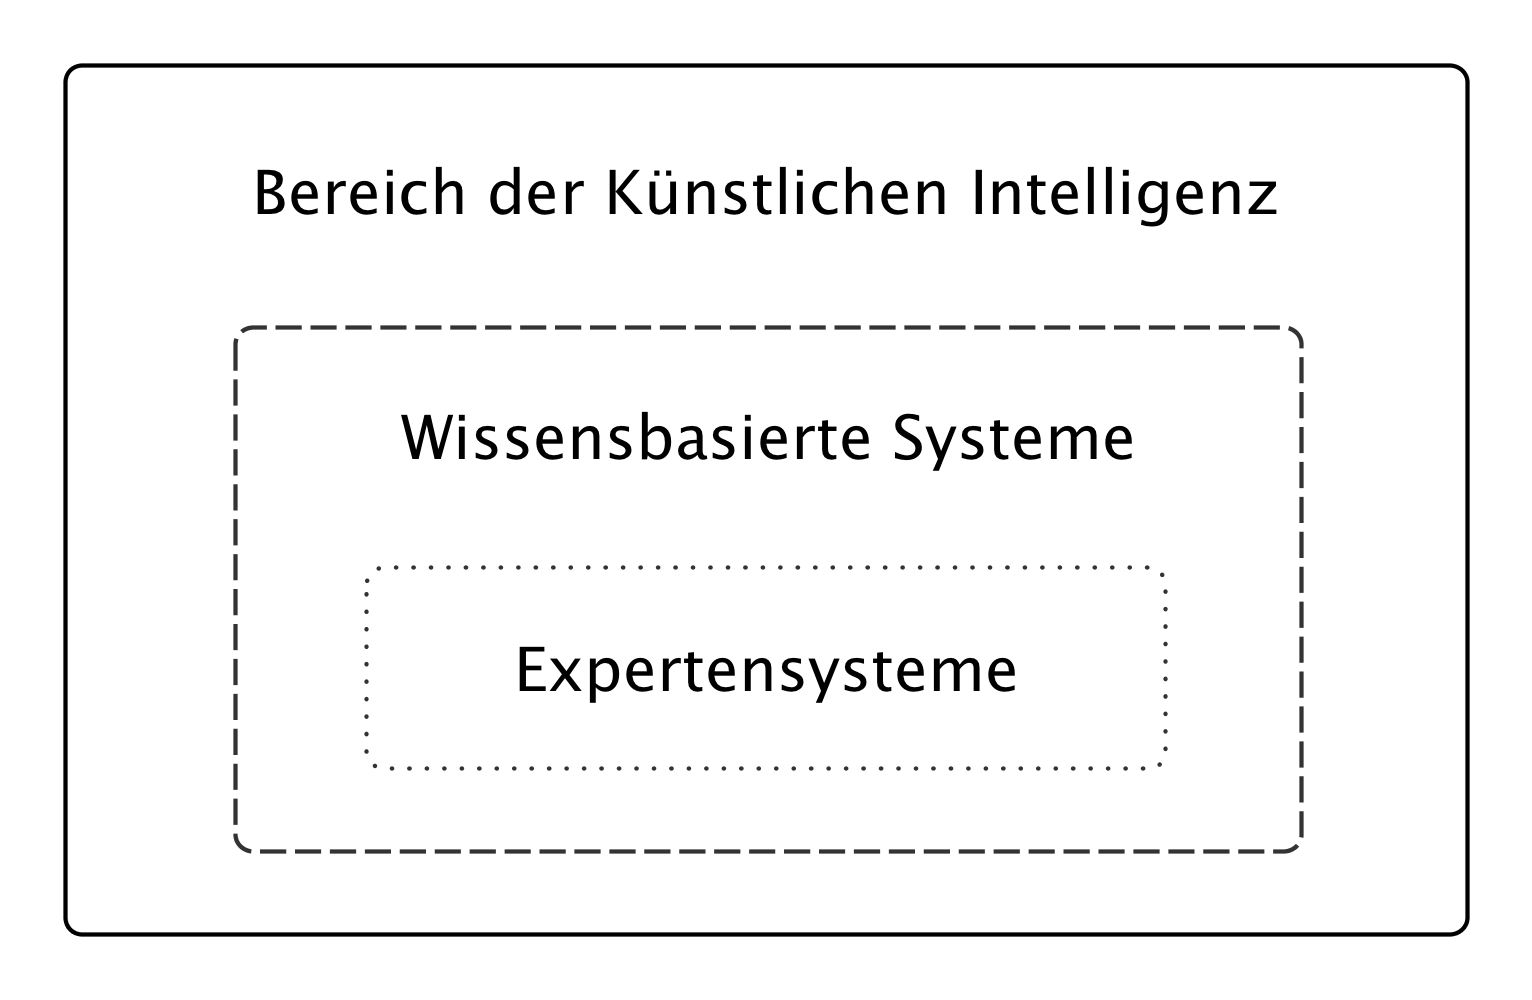
\includegraphics[width=0.55\textwidth]{images/abgrenzung.png}
	\caption{Begriffsabgrenzung, \cite[S.30]{haun2000}}
	\label{Abgrenzung}
\end{figure} 
Nach dieser Agbrenzung l�sst sich feststellen, dass der Unterschied zwischen einem Wissensbasierten System und einem Expertensystem darin besteht, dass das Wissen im Endeffekt von einem Experten stammt. Allerdings ist dieses Kriterium zu einfach und nicht besonders aussagekr�ftig. Beierle und Kern-Isberner weisen drauf hin, dass nach diesem Kriterium viele existierenden Wissensbasierten Systeme als Expertensysteme bezeichnet werden k�nnten \cite[S.11]{beierle2014}. Aufgrund dessen stellen die Autoren die Eigenschaften eines Experten dar, die sich folgenderma�en zusammenfassen lassen:
\begin{itemize}
\item Experten sind selten und teuer.
\item Experten sind nicht immer verf�gbar.
\item Leistungsf�higkeit der Experten ist nicht konstant, sondern kann nach Tagesverlauf schwanken.
\item Expertenwissen kann oft nicht als solches weitergegeben werden.
\item Expertenwissen kann verloren gehen.
\end{itemize}
Ein gutes Beispiel hinsichtlich der Gefahr, dass Expertenwissen verloren gehen kann, wird in \cite[S.94]{gebus2009} vorgestellt. Gebus nimmt den Bezug auf die Mitarbeiter der sogenannten Baby-Boomgeneration. Es handelt sich um Experten, die ein umfangreiches Erfahrungswissen besitzen und bald aus Altersgr�nden das Unternehmen verlassen. Somit geht auch das Erfahrungswissen aus dem Unternehmen verloren.\\
Zusammenfassend l�sst sich sagen, dass die Entwicklung eines Expertensystems eine hohes Potenzial besitzt. Allerdings kann ein Expertensystem nicht als Ersatz eines menschlichen Experten betrachtet werden. Vielmehr geht es um eine Erfassung, Darstellung und Pflege des Expertenwissens in einem Expertensystems, um die Arbeitsprozesse effizienter zu gestalten und sowohl erfahrene als auch neue Anwender in einem bestimmten Wissensbereich bei der Aufgabenabwicklung zu unterst�tzen.